%%%%%%%%%%%%%%%%%%%%%%%%%%%%%%%%%%%%%%%%%%%%%%%%%%%%%%%%%%%%%%%%%%%%%%%%%%%%%%
%
% Space Warps System Paper
%
%%%%%%%%%%%%%%%%%%%%%%%%%%%%%%%%%%%%%%%%%%%%%%%%%%%%%%%%%%%%%%%%%%%%%%%%%%%%%%

\documentclass[useAMS,usenatbib,a4paper]{mn2e}
%% letterpaper
%% a4paper

\voffset=-0.6in

% Packages:
\input psfig.sty
\usepackage{xspace}
\usepackage{graphicx}
\usepackage{amssymb}
\usepackage{amsmath}

% Macros:
% JOURNALS
\newcommand{\apj}{ApJ}
\newcommand{\apjl}{ApJL}
\newcommand{\apjs}{ApJS}
\newcommand{\mnras}{MNRAS}
\newcommand{\apss}{Ap \& SS}
\newcommand{\aap}{A\&A}
\newcommand{\aj}{AJ}
\newcommand{\prd}{Phys. Rev. D}
\newcommand{\nat}{Nature}
\newcommand{\araa}{ARA\&A}
\newcommand{\jgr}{J. Geophys. Res.}
\newcommand{\pasp}{PASP}

% MISC
\newcommand{\etal}{et~al.~}
\newcommand{\eg}{{\it e.g.\ }}
\newcommand{\ie}{{\it i.e.\ }}
\newcommand{\etc}{{\it etc.\ }}

\newcommand{\be}{\begin{equation}}
\newcommand{\ee}{\end{equation}}
\newcommand{\bea}{\begin{eqnarray}}
\newcommand{\eea}{\end{eqnarray}}


% CROSS-REFERENCING
\def\Sref#1{Section~\ref{#1}\xspace}
\def\Fref#1{Figure~\ref{#1}\xspace}
\def\Tref#1{Table~\ref{#1}\xspace}
\def\Eref#1{Equation~\ref{#1}\xspace}
\def\Aref#1{Appendix~\ref{#1}\xspace}

% UNITS
\newcommand{\kms}{\ifmmode  \,\rm km\,s^{-1} \else $\,\rm km\,s^{-1}  $ \fi }
\newcommand{\kpc}{\ifmmode  {\rm kpc}  \else ${\rm  kpc}$ \fi  }  
\newcommand{\pc}{\ifmmode  {\rm pc}  \else ${\rm pc}$ \fi  }  
\newcommand{\Msun}{\ifmmode {\rm M_{\odot}} \else ${\rm M_{\odot}}$ \fi} 
\newcommand{\Zsun}{\ifmmode {\rm Z_{\odot}} \else ${\rm Z_{\odot}}$ \fi} 
\newcommand{\yr}{\ifmmode yr^{-1} \else $yr^{-1}$ \fi} 
\newcommand{\hMsun}{\ifmmode h^{-1}\,\rm M_{\odot} \else $h^{-1}\,\rm M_{\odot}$ \fi}

% COSMOLOGY
\newcommand{\LCDM}{$\Lambda{\rm CDM}$}
\newcommand{\MS}{Millennium Simulation\xspace}

% LENSING
\def\zd{z_{\rm d}}
\def\zs{z_{\rm s}}
\def\Dd{D_{\rm d}}
\def\Ds{D_{\rm s}}
\def\Dt{D_{\Delta t}}
\def\Dds{D_{\rm ds}}
\def\Sigmacrit{\Sigma_{\rm crit}}
\def\REin{R_{\rm Ein}}
\def\MEin{M_{\rm Ein}}

% SOFTWARE/HARDWARE
\def\sw{{\small\sc Space\,Warps}\xspace}
\def\SW{{\sc Space\,Warps}\xspace}
\def\Talk{{\small\sc Talk}\xspace}
\def\Letters{{\small\sc Letters}\xspace}
\def\Letter{{\small\sc Letter}\xspace}
\def\Dashboard{{\small\sc Dashboard}\xspace}
\def\cfhtls{{\it CFHTLS}\xspace}
\def\python{{\sc python}\xspace}

% TABLES:
\newcommand\nodata{ ~$\cdots$~ }%

% PROBABILITY THEORY
\def\pr{{\rm Pr}}
\def\data{{\mathbf{d}}}
\def\datap{{\mathbf{d}^{\rm p}}}
\def\datai{d_i}
\def\datapi{d^{\rm p}_i}
\def\LENS{{\rm LENS}}
\def\saidLENS{{\rm ``LENS"}}
\def\NOT{{\rm NOT}}
\def\saidNOT{{\rm ``NOT"}}

% AGENT BUREAUCRACY
\def\effort{N_{\rm C}}
\def\experience{N_{\rm T}}
\def\skill{\langle I \rangle}
\def\contribution{$\sum_k \skill_k$}
\def\information{\delta I}

% COMMENTING
\usepackage[usenames]{color}
\newcommand{\question}[2]{\textcolor{red}{\bf Question from #1: #2}}
\newcommand{\flag}[2]{\textcolor{blue}{\bf Comment from #1: #2}}
\newcommand{\new}[1]{{\bf #1}}

% RESULTS
\def\Ncollaboration{XXX}

\def\oxford{Dept.\ of Physics, University of Oxford, Keble Road, Oxford, OX1 3RH, UK}
\def\oxfordeng{Dept.\ of Engineering Science, University of Oxford, Parks Road, Oxford, OX1 3PJ, UK}
\def\kipac{Kavli Institute for Particle Astrophysics and Cosmology, Stanford University, 452 Lomita Mall, Stanford, CA 94035, USA}
\def\ipmu{Kavli IPMU (WPI), University of Tokyo, 5-1-5 Kashiwanoha, Kashiwa 277-8583, Japan}
\def\zooniverse{Zooniverse, c/o Astrophysics Department, University of Oxford, Oxford OX1 3RH, UK}
\def\adler{Adler Planetarium, Chicago, IL, USA}
\def\lausanne{EPFL, Lausanne, Switzerland}
\def\zurich{Department of Physics, University of Zurich, Switzerland}
\def\paris{Institut d’Astrophysique de Paris, UMR7095 CNRS – Universit\'e Pierre et Marie Curie, 98bis bd Arago, 75014 Paris, France}
\def\icg{Institute of Cosmology and Gravitation, University of Portsmouth, Dennis Sciama Building, Portsmouth P01 3FX, UK}

\def\pjmemail{\tt pjm@slac.stanford.edu}
\def\amemail{\tt anupreeta.more@ipmu.jp}


\def\indic#1{\mathbb{I}\left({#1}\right)}

%%%%%%%%%%%%%%%%%%%%%%%%%%%%%%%%%%%%%%%%%%%%%%%%%%%%%%%%%%%%%%%%%%%%%%%%%%%%%%

\title[\sw]
{\SW Extended! Snappy Titles!}

\author[Davis et al.]{%
  % The \SW Collaboration includes:

% Principal Investigators (opt-out):
   \newauthor{%
    Philip~J.~Marshall,$^{1,2}$\thanks{\pjmemail}
    Aprajita~Verma,$^{2}$
    Anupreeta~More,$^{3}$
    Christopher~P.~Davis,$^{1}$
    }
    \newauthor{%
    Surhud~More,$^{3}$
    Amit~Kapadia,$^{4}$
    Michael~Parrish,$^{4}$
    Chris~Snyder,$^{4}$
    }
   \newauthor{%
    Julianne~Wilcox,$^{5}$
    Elisabeth~Baeten,$^{5}$
    Christine~Macmillan,$^{5}$
    Claude~Cornen,$^{5}$
    }
   \newauthor{%
    Michael~Baumer,$^{1}$
    Edwin~Simpson,$^{6}$
    Chris~J.~Lintott,$^{2}$
    David~Miller,$^{4}$
    }
   \newauthor{%
    Edward~Paget,$^{4}$
    Robert~Simpson,$^{2}$
    Arfon~M.~Smith,$^{4}$
    Rafael~K\"ung,$^{7}$
    }
   \newauthor{%
    Prasenjit~Saha,$^{7}$
    Thomas~E.~Collett$^{8}$
    }
 %
\medskip\\
$^1$\kipac\\
$^2$\oxford\\
$^3$\ipmu\\
$^4$\adler\\
$^5$\zooniverse\\
$^6$\oxfordeng\\
$^7$\zurich\\
$^8$\icg\\

}

%%%%%%%%%%%%%%%%%%%%%%%%%%%%%%%%%%%%%%%%%%%%%%%%%%%%%%%%%%%%%%%%%%%%%%%%%%%%%%

\begin{document}

\date{to be submitted to ?!?!}
\pagerange{\pageref{firstpage}--\pageref{lastpage}}\pubyear{2014}

\maketitle

\label{firstpage}

%%%%%%%%%%%%%%%%%%%%%%%%%%%%%%%%%%%%%%%%%%%%%%%%%%%%%%%%%%%%%%%%%%%%%%%%%%%%%%

\begin{abstract}

\todo{Chris}{Do abstract!}

\end{abstract}

% Full list of options at http://www.journals.uchicago.edu/ApJ/instruct.key.html

\begin{keywords}
  gravitational lensing   --
  methods: statistical    --
  methods: citizen science
\end{keywords}

\setcounter{footnote}{1}

%%%%%%%%%%%%%%%%%%%%%%%%%%%%%%%%%%%%%%%%%%%%%%%%%%%%%%%%%%%%%%%%%%%%%%%%%%%%%%

\section{Introduction}
\label{sec:intro}


% \section{Introduction}
% \label{sec:intro}
% \section{Offline \SW}
% \label{sec:offline}
% \subsection{Formalism}
% \label{sec:offline:formalism}
% \subsection{Training}
% \label{sec:design:training}
% \section{Results}
% \label{sec:results}
% \section{Discussion}
% \label{sec:discuss}
% \section{Conclusions}
% \label{sec:conclude}

%%%%%%%%%%%%%%%%%%%%%%%%%%%%%%%%%%%%%%%%%%%%%%%%%%%%%%%%%%%%%%%%%%%%%%%%%%%%%%

\section{Dataset}

%%%%%%%%%%%%%%%%%%%%%%%%%%%%%%%%%%%%%%%%%%%%%%%%%%%%%%%%%%%%%%%%%%%%%%%%%%%%%%

% TODO:
% Kamal Nigam, Andrew McCallum and Tom Mitchell. Semi-supervised Text Classification Using EM. In Chapelle, O., Zien, A., and Scholkopf, B. (Eds.) Semi-Supervised Learning. MIT Press: Boston. 2006.
% according to
% http://www.mblondel.org/journal/2010/06/21/semi-supervised-naive-bayes-in-python/#more-126
% this paper would be an example of the sort of thinking I had with the EM
% algorithm (not quite what was implimented in stage 2 at phil's request),
% where the E step just does the unlabeled, and the M step uses both labeled
% and unlabeled data

\section{Formalism}
\label{sec:formalism}

\todo{Chris}{This section will describe the different ways we can use the data
  we got from SpaceWarps to do a beter job with classifications. So we can then
  look at the way SpaceWarps updates the PL, PD, and p's of the objects, either
  via offline, using both/either/neither training and test data (in either online or offline
contexts), manipulating initializations, etc. We could also see what the
benefits are for using the known lens information. Finally, we should examine the
benefits of using a validation dataset (using information we already have!) to
improve our estimates.}
\flag{Chris}{I don't like using $p^0$ to both represent the true prior prior
and our estimate of the correct prior according to the EM algorithm.}

\sw keeps track of the following parameters:
\begin{itemize}
  \item{$C_{ij}$, the classification the $i$-th volunteer made of the $j$-th
      image. $C_{ij}$ may take on three values:
      0, 1, or empty. Since volunteers do not see most images, the vast
    majority of $C_{ij}$ are blank.}
    \item{$PD_{i}$, the probability, given that the image is a dud, that
        $i$-th the volunteer will classify it as a dud. The
      probability, given that the image is a dud, that the volunteer will
    classify it as a lens follows as $1 - PD_{i}$.}
  \item{$PL_{i}$, the probability, given that the image is actually a
      lens, that the $i$-th volunteer will classify it as being a lens. The
      probability, given that the image is a lens, that the volunteer will
    classify it as a dud follows as $1 - PL_{i}$.}
  \item{$p_j$, the probability that
      the $j$-th image $z_{j}$ is a lens given the current observations and skills of the
  volunteers who classified it.}
  \item{$p^{0}$, the prior probability that an object is a lens.}
\end{itemize}

% % % % % % % % % % % % % % % % % % % % % % % % % % % % % % % % % % % % % % %

\subsection{The Online System}
\label{sec:formalism:online}
In \sw, this is fixed at $2 \times 10^{-4}$, or the expectation that
around 100 lenses will be found in 430,000 images. Because \sw is an online
system that constantly reevaluates most of the above parameters (except $p_0$
and any non-blank $C_{ij}$) in order to promote likely lenses\footnote{Note
that this does not change the probability that a volunteer will actually draw
said image.} or to retire likely duds,\footnote{Images whose probability of
being a lens drops below a certain threshold are removed from the active
dataset.} we augment $p$, $PL$, and $PD$ as $p_j^k$, the evaluation of
$p_j$ at time $k$. \sw uses Bayes' Theorem to update $p_j^{(k + 1)}$ for
some new evaluation $C_{ij}$\footnote{There is no superscript for $C_{ij}$
because each user only sees an image once.}:
\begin{align}
  p_j^{(k + 1)} &= \left ( \frac{C_{ij} PL_{i}^{k}
  }{PL_{i}^{k} p_j^k + (1 - PD_{i}^{k})(1 -
  p_j^k)}
  \right. \notag \\ & \; \left . +
  \frac{(1 - C_{ij}) (1 - PL_{i}^{k})
  }{(1 - PL_{i}^{k}) p_j^k + PD_{i}^{k}(1 -
  p_j^k)} \right ) p_j^k \ ,
\end{align}
The first term on the right hand side is the probability update for evaluating
the object to be a lens, while the second term is the probability that the
image is a lens if the volunteer evaluates it to be a dud.  (For example, an
obtuse volunteer who always perfectly incorrectly classifies an image will
actually change the probability exactly the same as one who always perfectly
correctly classifies an image, given that the estimate of the obtuse
volunteer's skill ($PL_{i} = 0$) is accurate.)

\sw only updates the volunteer's $PL_{i}$ and $PD_{i}$ after volunteer $C_i$
classifies a training image:

\begin{align}
  PL_{i}^{(k + 1)} &= \frac{PL_{i}^{k} (NL_{i}^{k} + M) + \mathbb{I}[C_{ij} =
  z_{j}]}{NL_{i}^{k} + M + z_{j}} \\
  PD_{i}^{(k + 1)} &= \frac{PD_{i}^{k} (ND_{i}^{k} + M) + \mathbb{I}[C_{ij} =
  z_{j}]}{ND_{i}^{k} + M + z_{j}}
\end{align}
where $ND_{i}^{k}$ and $NL_{i}^{k}$ refer to the number of training lenses and
training duds observed by the $i$-th volunteer at time $k$, $z_{j}$ refers to
the true state of the $j$-th image (1 is LENS, 0 is DUD), and $M = 4$ is a
smoothing factor empirically derived to smooth the skill classification of new
volunteers.

With these update rules plus an initialization of $PD_{i} = PL_{i} = 0.5$ and
$p^{0} = 2 \times 10^{-4}$, the online update system is fully specified.

% % % % % % % % % % % % % % % % % % % % % % % % % % % % % % % % % % % % % % %

\subsection{An Offline Expectation Maximization Approach}
\label{sec:formalism:em}
Using the above notation but expanding $p^{0}$ to $p_{ij}^{0}$ (allowing, e.g. for
the distribution of training images to differ for each volunteer, perhaps based on
the number of images they have observed, or to allow a particular image to be
more likely to be drawn), the complete log-likelihood for this model may be
specified:
\begin{multline}
  \mathrm{CLL}(C_{ij}, z_{j}, PL_{i}, PD_{i}, p_{ij}^{0}) \\ = \sum_{i} \sum_{j \in \Omega_i} C_{ij} z_{j} \log PL_{i} +
      (1 - C_{ij}) z_j \log (1 -
      PL_{i}) \\ + (1 - C_{ij}) (1 - z_j) \log PD_{i} + C_{ij} (1 - z_j) \log (1 - PD_{i}) \\ + z_j \log p_{ij}^{0} +
      (1 - z_j ) \log(1 - p_{ij}^{0})
\end{multline}
where $\Omega_i$ is the set of all images volunteer $i$ has observed in $\Omega$,
the set of all images in the program.\footnote{Because the probability that a
  viewer views a given image (given it is a training or test image) is random,
I choose to simply ignore the unobserved images.} We can use this complete
log-likelihood to derive an offline expectation maximization algorithm for
determining the lens probabilities, user skills, and lens priors.

% % % % % % % % % % % % % % % % % % % % % % % % % % % % % % % % % % % % % % %

\subsubsection{E-Step}
\label{sec:formalism:em:estep}
% TODO: reword. The maximization here is over the zj's, so word to make that clear.
% The E-Step is just taking the expected complete log-likelihood, or the
% expectation value over $P(\cdot \ | x, \phi)$.
The E-Step is maximizing the complete log-likelihood with respect to the image
probability $p_j$.  This is equivalent to replacing $z_j$ with $p_j$:
% TODO: replace this with equivalent like eq1
\begin{align}
  p_j &= \frac{1}{N_j} \sum_{i \in \Omega_j} P(z_j = 1 \ | \ C_{ij} ; \Phi) =
  \frac{1}{N_j} \sum_{i \in \Omega_j} \frac{ P(C_{ij} \ | \ z_j = 1; \Phi)
P(z_j = 1 ; \Phi)}{P(C_{ij} ; \Phi)} \\
&= \frac{1}{N_j} \sum_{i \in \Omega_j} \frac{ PL_{i}^{C_{ij}} (1 - PL_{i})^{(1 -
C_{ij})} p_{ij}^{0}}{ PL_{i}^{C_{ij}} (1 -
  PL_{i})^{(1 - C_{ij})} p_{ij}^{0} + PD_{i}^{(1 - C_{ij})} (1 -
PD_{i})^{C_{ij}} (1 - p_{ij}^{0})}
\end{align}
where $i \in \Omega_j$ is now the set of classifications done on the $j$-th
image and $N_j$ is the number of classifications done on the $j$-th image. This
makes sense: $p_{ij}^{0}$ is just the prior likelihood of an image being a lens,
while $PL_{i}$ is how well we would have identified a lens as such.

% % % % % % % % % % % % % % % % % % % % % % % % % % % % % % % % % % % % % % %

\subsubsection{M-Step}
\label{sec:formalism:em:mstep}
The M-Step is done by maximizing the expected complete log-likelihood with
regard to the input parameters $PD_{i}, PL_{i}, p_{ij}^{0}$. Doing the
maximization process, we find:
\begin{align}
  PL_{i} &= \frac{\sum_{j \in \Omega_i} C_{ij} p_{j}}{\sum_{j \in
\Omega_i} p_{j}} \\
  PD_{i} &= \frac{\sum_{j \in \Omega_i} (1 - C_{ij}) (1 - p_{j})}{\sum_{j \in
\Omega_i} (1 - p_{j})}
\end{align}
\begin{align}
  p_{ij}^{0} &= p_{j} \ , &p_{i}^{0} = \frac{\sum_{j \in \Omega_i}
p_{j}}{\sum_{j \in \Omega_i} 1} \notag\\
   p_{j}^{0} &= p_{j} \ , &p^{0} = \frac{\sum_i \sum_{j \in \Omega_i}
p_{j}}{\sum_i \sum_{j \in
  \Omega_i} 1} \ ,
\end{align}
where the possible specializations of $p_0$ are also given. These mirror quite
closely the online systems, except that skill is now assessed against
the majority expectation of the probability of an image being a lens, instead
of its true value.

In practice we have training images where $p_{j}$ is known. In those
cases we can use the true value when doing the M-Step. We can also choose to
perform the M-step using only the training images (a supervised learning
approach), giving us another handle on quantifying the impact and importance of
simulated training images.

Finally, we also include Laplace smoothing into the M-Step in order to handle
pathologic cases, such as when users never identify any lenses ($\sum_{j \in
\Omega_{i}} p_j = 0$). The estimators for $PL_{i}$ and $PD_{i}$ now become:
\begin{align}
  PL_{i} &= \frac{M + \sum_{j \in \Omega_i} C_{ij} p_{j}}{2M + \sum_{j \in
\Omega_i} p_{j}} \\
  PD_{i} &= \frac{M + \sum_{j \in \Omega_i} (1 - C_{ij}) (1 - p_{j})}{2M + \sum_{j \in
\Omega_i} (1 - p_{j})}
\end{align}
where for Laplace smoothing, $M = 1$.

We choose to specialize $p^{0}$ to vary with
image, $p_{j}^{0}$, because images are taken out of the \sw system if they reach
too low a probability, clearly changing the prior when we evaluate at the end
of the run; training images also have a
different prior on being a lens as well. Finally, if the image is a training
image with known $p_j \in (0,1)$, then the known $p_j$ is used instead of
the current estimate.

An easy way to conceptualize the previous section is to note that the
Expectation Maximization takes advantage of the fact that each classification
is supposed to be independent of the others and so can be treated as though all
classifications were made at the same time.  The repetition of the steps
ensures that the parameters are self-consistent.

% % % % % % % % % % % % % % % % % % % % % % % % % % % % % % % % % % % % % % %

\subsection{Validation of Training}
\label{sec:validation}

\todo{Chris}{In order to look at a validation dataset, I need to create a
  blacklist of agents and subjects (and decide what sort of division of either
/ both / neither constitutes a good validation dataset here) that SWAP.py can
then read in and process.}

A validation dataset is needed to prevent overfitting training data and to try
to test how the training data does against real lenses. These need to come in
two categories: actual lens environments, and simulated lenses. The need for
two sets arises because of the paucity of actual lenses. In \SW, most training
objects are explicitly given to a user -- if a user incorrectly identifies a
training object, they are informed of that failure, and likewise for a correct
classification.

Problems:
0. By telling users about failures in the sim/dud, we explicitly break the
notion that users come in fully-formed. But we also need to give users
incentives to keep working, by rewarding them for good behavior. Replace by
current crowd assessments and telling them how they did compared with the
crowd?
1. \SW does not have any 'silent' training images which could function as
validation datasets, since you have broken the training by telling users.
2. How to manage the difference between 'dud known lens fields' and 'dud sim
fields'? Just put them together?
3. If you tell users about the correct sim classification, do you also tell
them about a correct lens classification, and do you tell them it was a real
lens?
4. Can I just use the dud fields?

% % % % % % % % % % % % % % % % % % % % % % % % % % % % % % % % % % % % % % %

\subsection{Expanding Number of Classifications}
\todo{Chris}{In this section, we expand possible classifications from LENS and
  NOT to, say 0, 1, 2, 3. In effect, I take the stuff of \ref{sec:formalism:em}
  and extend it to a multinomial model. I should put in the generative model
here as well as the new confusion matrix. I have written the first several
steps below (not properly formatted and all that).}

\flag{Chris}{In the below formalism everything can only be classified once.
  That is, classification from user $i$ on subject $j$ as type $u$ is $C_{ij} =
  u$. If we want to expand classification numbers, we could say instead
$C_{iju} = 1$ for 1 classification as type $u$. Then, if you draw $M$ total
classifications, you replace $\text{Uniform}\left(p\right)$ with
$\text{Mult}\left(p, M\right)$. \\
Now you may ask: Chris, why would we ever make more than one classification on
a subject? And I would agree, except that this provides an avenue for analyzing
how to use \SW to deal with the markers (where there usually are multiple classifications).}

We can extend the \SW binomial model to include multiple classifications and
multiple categories -- we can talk about things like $P(``1" | \rm{LENSED\
QUASAR})$ where a user assigns an object a rank $"1"$ and wish to know the
likelihood that a lensed quasar would yield that category.

Unfortunately our $PL$ and $PD$ terms must be
generalized. We introduce instead $P_{ivu}$ to represent the $i$-th user's
probability of making classification $``u"$ given that the object is of type
$v$: $P_{ivu} = P(``u" | v)_i$. Naturally, the conditional probabilities are
normalized over the possible classifications $``u"$: $\sum_u^U P_{ivu} = 1$. Overall there are $U$ types of
classifications a user can make, representing $V$ types of objects.

We also must expand $p^0$ to represent more than a binary classification.
$p_{jv}^0$ is the prior probability that object $j$ is of type $v$. Naturally,
$\sum_v p_{jv}^0$ = 1.
The latent variable of subject $j$ as object $v$ is $z_{jv} = 1$ with all
other $z_{jv} = 0$. Similarly, the classification of user $i$ on subject $j$
as type $u$ is $C_{iju} = 1$ with all other $C_{iju} = 0$.
% The latent variable of subject $j$ as object $v$ is $z_{j} =
% v$. Similarly, the classification of user $i$ on subject $j$ as type $u$ is
% $C_{ij} = u$.

This is our generative model with explicit latent variables:
\begin{itemize}
  \item{Draw latent subject indicator vectors from the prior probability: $$z_{j}
    \overset{\text{iid}}{\sim} \text{Uniform}\left(p^0\right)$$}
  \item{Given latent subject indicator $z_{j}$ and the $i$-th user's confusion
    matrix $P_i$, independently draw a classification vector from the $z_j$-th column
  of $P_i$: $$C_{ij} | z_{j} \overset{\text{ind}}{\sim}
\text{Uniform}\left(P_{i,z_j}\right)$$}
\end{itemize}
Hence, we can also make the following statements:
\begin{equation}
  p(z_{jv}) = p^0_{jv}
\end{equation}
% equiv: p(z_j = v) = p^0_v
\begin{equation}
  \label{eq:PCiju}
  P(C_{iju} | z_{jv}; p^0_{jv}, P_{ivu}) = P_{ivu}^{C_{iju}}
\end{equation}

Thus our complete log likelihood is (ignoring irrelevant normalization terms)
% \begin{align}
%   \log p \left( C_{ij}, z_{j}; p_{jv}^0, P_{ivu} \right) &\propto
%                                                       \sum_{i} \sum_{j \in
%                                                       \Omega_i} \indic{z_j = v}
%                                                       \log p_{jv}^0 \notag\\
% &+ \indic{C_{ij} = u} \indic{z_j = v} \log P_{ivu}
% \end{align}
% where $\indic{}$ is the indicator function which evaluates as one when the
% contained statement is true and zero when it is false.
% \flag{Chris}{If you want to write it without indicators, expand the notation to
%   vectors and you get the following:}
\begin{align}
  \log p \left( C_{iju}, z_{jv}; p_{jv}^0, P_{ivu} \right) &\propto \sum_{i} \sum_{j \in
\Omega_i} \sum_{v} z_{jv} \log p_{jv}^0
  \notag\\
  &+ \sum_{i} \sum_{j \in \Omega_i} \sum_{v} \sum_{u} C_{iju} z_{jv} \log P_{ivu}
\end{align}

\subsubsection{E-Step}

Now we repeat the exercise earlier of computing the expected complete log
likelihood under the conditional distribution $p(z_{j} | C_{ij}; p^0,
P_{i})$. Call $p_{jv} = p(z_{jv} | C_{iju}; p^0_{jv}, P_{ivu})$. It is
sufficient to compute $p_{jv}$ to complete this step. By Bayes's Rule, we
know that
\flag{Chris}{Is this an abuse of notation? I want for a single $z_{jv}$, but
given $C_{iju}, p^0_{jv}, P_{ivu}$ for \textit{all} $i$ and $u$. So really it
is more correct to say $ p(z_{jv}) \prod_i \prod_u p(C_{iju} | z_{jv}; p^0_{jv},
P_{ivu})$ since each classification $C_{ij}$ is independent. Should I do that?
Alternatively, I could put one of those $\cdot$ in place of each $i$ and $u$...}
$$
p(z_{jv} | C_{iju}; p^0_{jv}, P_{ivu}) \propto p(C_{iju} | z_{jv}; p^0_{jv},
P_{ivu}) p(z_{jv})
$$
But we know the values of all these terms, so we find:
\todo{Chris}{Double check this. I'm not sure it's strictly correct when you
have more than one classification per image / type.}
\begin{align}
  p_{jv} = \frac{1}{N_j} \sum_{i \in \Omega_j} \frac{\prod_u p^0_{jv}
  P_{ivu}^{C_{iju}}}{\sum_{v'} \prod_u p^0_{jv'} P_{iv'u}^{C_{iju}}}
\end{align}

\subsubsection{M-Step}

We maximize the expected complete log likelihood. This is straightforwardly
\todo{Chris}{Maybe not so straightforwardly if you have multiple
classifications. Check that!}
\begin{align}
  P_{ivu} &= \frac{\sum_{j \in \Omega_i} C_{iju} p_{jv}}{\sum_{j \in
\Omega_i} p_{jv}} \\
  p_{jv}^0 &= p_{jv} \\
  p_{v}^0 &= \frac{\sum_i \sum_{j \in \Omega_i} p_{jv}}{\sum_i \sum_{j \in
\Omega_i} 1}
\end{align}
where $p_{v}^0$ is a possible specialization of $p_{jv}^0$.

\subsubsection{Online}

Like in the binomial case, the multinomial case can be performed online, where
each new piece of information updates an existing assessment of lens
classification and user skill. If a new classification $C_{iju}^{(k + 1)}$ is
made, then by Bayes' Theorem the updates are as follows (with $i$, $j$, $u$,
and $v$ acting as fixed indices):
\begin{align}
  p_{jv}^{(k + 1)} &= \left( \frac{P^{k}_{ivu}^{C_{iju}^{(k + 1)}}}{\sum_{v'}
  p_{jv'}^{k} P^{k}_{iv'u}^{C_{iju}^{(k+1)}}} \right) p_{jv}^{k} \\
  P^{(k+1)}_{ivu}  &= \frac{C^{(k+1)}_{iju} p^{k}_{jv} + P^{k}_{ivu} \sum_{j'\in
  \Omega_i} p^{k}_{j'v} }{p^{k}_{jv} + \sum_{j'
  \in \Omega_i} p^{k}_{j'v}}
\end{align}
If we are using only a supervised learning set, then $p^k_{j'v} \in (0, 1)$.

\subsubsection{Checks}
\todo{Chris}{This section will make some obvious checks on the generalized
  model. First I should be able to write down the binary model using this
  formalism. Next, I should be able to show for sure that different $u$ can
lead to different probability assignments if $v$ can only be two categories --
that is, I should be able to show that $`1'$ gives a mixture of probability for
LENS and NOT that makes sense when compared with $`0'$ or $`2'$. \\
This section can probably be removed. This is more for internal sharing to help
keep everyone up to speed.}

Let's make sure we recover the old system. In our new notation, $u$ could be
"LENS" or "NOT" while $v$ could be LENS or NOT. So, $PL_i = P_{iLL}$ and $PD_i
= P_{iNN}$. We use the conservation of total probability to note that
$P_{iLN} = 1 - P_{iLL} = 1 - PL_i$ and $P_{iNL} = 1 - P_{iNN} = 1 -
PD_i$. Meanwhile, $p_j^0$ becomes $p_{jL}^0$ and we use conservation of total
probability to note that $p_{jN}^0 = 1 - p_{j}^0$. We now account for the
labels: $z_{j} = z_{jL}$ and $z_{jN} = 1 - z_{j}$. (There can only be one
label on these objects.) Similarly for the classifications: $C_{ij} = C_{ijL}$,
so $C_{ijN} = 1 - C_{ij}$.

We can hence expand the
sums over $v \in (L, N)$ and $u \in (L, N)$ to find that our CLL is
proportional to:
\begin{align}
z_{jL} \log p_{jL}^0 + z_{jN} \log p_{jN}^0 +
C_{ijL} z_{jL} \log P_{iLL} + C_{ijN} z_{jL} \log P_{iLN} \notag\\ + C_{ijL} z_{jN} \log
P_{iNL} + C_{ijN} z_{jN} \log P_{iNN} = \notag\\
z_j \log p_j^0 + (1 - z_j) \log (1 - p_j^0) + C_{ij} z_j \log PL_i + (1 -
C_{ij}) z_j \log (1 - PL_i) \notag\\
+ C_{ij} (1 - z_j) \log (1 - PD_i) + (1 - C_{ij})
(1 - z_j) \log PD_i
\end{align}
which is the same CLL as before.

% % % % % % % % % % % % % % % % % % % % % % % % % % % % % % % % % % % % % % %

\section{Dynamic Allocations}
\todo{Chris}{This section will examine whether we would be better off
  dynamically assigning images to people (based on current estimates of skill
  and probability) rather than randomly assigning them. This means I will need
  to create some sort of 'SpaceWarps Emulator'. (Actually, the other thing
  I can do is use the blacklist developed earlier to throw out
  contributions in an informed manner in order to construct different
  simulations.) Before I even do that, another
aspect I would like to examine and is probably useful is whether we can
reliably identify skilled users early on. That is, instead of looking at final
skill vs effort, look at many trajectories of skill vs effort over time. That
would be a useful thing to show to prove that we can find the good users in the
first place -- early on!}

% % % % % % % % % % % % % % % % % % % % % % % % % % % % % % % % % % % % % % %

\section{Discussion}

\section{Conclusions}

% %%%%%%%%%%%%%%%%%%%%%%%%%%%%%%%%%%%%%%%
% \begin{figure*}
% %\centering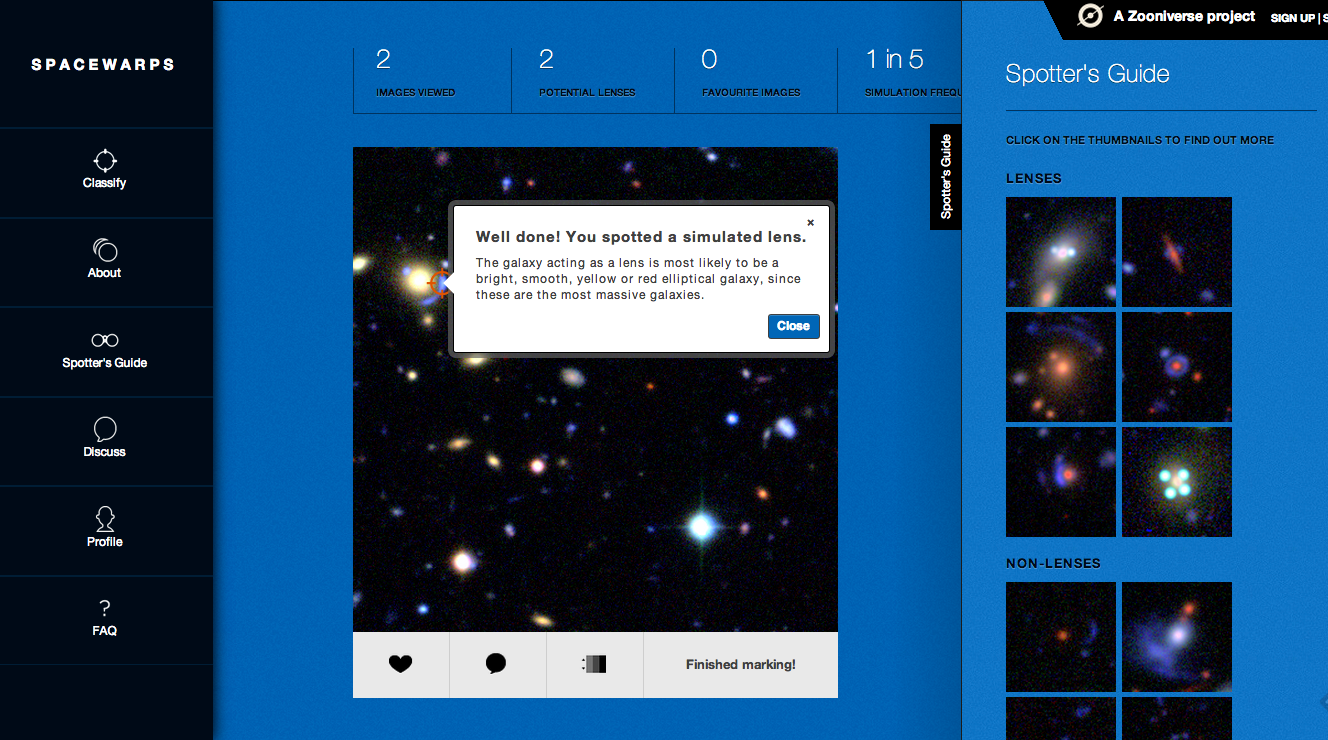
\includegraphics[width=0.9\linewidth]{sw-system-figs/sw-screengrab-marker+feedback.png}
% \caption{Screenshot of the \sw classification interface.}
% \label{fig:screenshot}
% \end{figure*}
% %%%%%%%%%%%%%%%%%%%%%%%%%%%%%%%%%%%%%%%

%%%%%%%%%%%%%%%%%%%%%%%%%%%%%%%%%%%%%%%%%%%%%%%%%%%%%%%%%%%%%%%%%%%%%%%%%%%%%%
%%  ACKNOWLEDGMENTS
%%%%%%%%%%%%%%%%%%%%%%%%%%%%%%%%%%%%%%%%%%%%%%%%%%%%%%%%%%%%%%%%%%%%%%%%%%%%%%

\section*{Acknowledgements}

% We thank all \Ncollaboration members of the \sw community for their
contributions to the project so far. A complete list of collaborators is
provided at \texttt{http://spacewarps.org/\#/results/CFHTLS}.

We are also grateful to Stuart Lynn, Kelly Borden, Laura Whyte, Brooke Simmons,
David Hogg, Thomas Jennings, Layne  Wright, Cecile Faure, Jonathan Coles, Stuart
Lowe and Jean-Paul Kneib for many useful conversations about citizen science and
gravitational lens detection, and to the Dark Energy Survey and Pan-STARRS strong
lensing science teams for their suggestions and encouragement.

PJM was given support by the Royal Society, in the form of a research
fellowship, and by the U.S. Department of Energy under contract number DE-AC02-76SF00515.
%
AV acknowledges support from the Leverhulme Trust in the form of a research
fellowship.
%
The work of AM and SM was supported by World Premier International Research
Center Initiative (WPI Initiative), MEXT, Japan. The work of AM was also supported in
part by National Science Foundation Grant No. PHYS-1066293 and the hospitality
of the Aspen Center for Physics.
%
% Zooniverse / Sloan Foundation.
%
% Other authors.
PJM and ES thank the Institute of Astronomy and Astrophysics, Academia Sinica
(ASIAA) and Taiwan's Ministry of Science and Technology (MOST) for their
financial support of the workshop ``Citizen Science in Astronomy'' in March
2014, at which some parts of the SWAP analysis was developed.

The \sw project is open source.
The web app was developed at \texttt{https://github.com/Zooniverse/Lens-Zoo}, and was supported by a grant from the Alfred P. Sloan Foundation, 
while the SWAP analysis software was developed at
\texttt{https://github.com/drphilmarshall/SpaceWarps}.

The CFHTLS data used in this work are based on observations obtained with
MegaPrime/MegaCam, a joint project of CFHT and CEA/IRFU, at the
Canada-France-Hawaii Telescope (CFHT) which is operated by the National Research
Council (NRC) of Canada, the Institut National des Science de l'Univers of the
Centre National de la Recherche Scientifique (CNRS) of France, and the
University of Hawaii. This work is based in part on data products produced at
Terapix available at the Canadian Astronomy Data Centre as part of the
Canada-France-Hawaii Telescope Legacy Survey, a collaborative project of NRC and
CNRS.


%%%%%%%%%%%%%%%%%%%%%%%%%%%%%%%%%%%%%%%%%%%%%%%%%%%%%%%%%%%%%%%%%%%%%%%%%%%%%%
%  APPENDICES
%%%%%%%%%%%%%%%%%%%%%%%%%%%%%%%%%%%%%%%%%%%%%%%%%%%%%%%%%%%%%%%%%%%%%%%%%%%%%%

\appendix

%%%%%%%%%%%%%%%%%%%%%%%%%%%%%%%%%%%%%%%%%%%%%%%%%%%%%%%%%%%%%%%%%%%%%%%%%%%%%%



%%%%%%%%%%%%%%%%%%%%%%%%%%%%%%%%%%%%%%%%%%%%%%%%%%%%%%%%%%%%%%%%%%%%%%%%%%%%%%
%  REFERENCES
%%%%%%%%%%%%%%%%%%%%%%%%%%%%%%%%%%%%%%%%%%%%%%%%%%%%%%%%%%%%%%%%%%%%%%%%%%%%%%

% MNRAS does not use bibtex, input .bbl file instead.
% Generate this in the makefile using bubble script in scriptutils:

% bubble -f paper-lcr.tex references.bib
% \input{paper-lcr.bbl}

\bibliographystyle{apj}
\bibliography{references}


%%%%%%%%%%%%%%%%%%%%%%%%%%%%%%%%%%%%%%%%%%%%%%%%%%%%%%%%%%%%%%%%%%%%%%%%%%%%%%

\label{lastpage}
\bsp

\end{document}

%%%%%%%%%%%%%%%%%%%%%%%%%%%%%%%%%%%%%%%%%%%%%%%%%%%%%%%%%%%%%%%%%%%%%%%%%%%%%%
